\documentclass[12pt, psamsfonts]{amsart}

%-------Packages---------
\usepackage{amssymb,amsfonts}
\usepackage{fullpage}
\usepackage{tikz-cd}
\usepackage{todonotes}
\usepackage{physics}
\usepackage[all,arc]{xy}
\usepackage{enumerate}
\usepackage{enumitem}
\usepackage{mathrsfs}
\usepackage{theoremref}
\usepackage{graphicx}
\usepackage[bookmarks]{hyperref}

%--------Theorem Environments--------
%theoremstyle{plain} --- default
\newtheorem{thm}{Theorem}[section]
\newtheorem{cor}[thm]{Corollary}
\newtheorem{prop}[thm]{Proposition}
\newtheorem{lem}[thm]{Lemma}
\newtheorem{conj}[thm]{Conjecture}
\newtheorem{quest}[thm]{Question}

\theoremstyle{definition}
\newtheorem{defn}[thm]{Definition}
\newtheorem{defns}[thm]{Definitions}
\newtheorem{con}[thm]{Construction}
\newtheorem{exmp}[thm]{Example}
\newtheorem{exmps}[thm]{Examples}
\newtheorem{notn}[thm]{Notation}
\newtheorem{notns}[thm]{Notations}
\newtheorem{addm}[thm]{Addendum}
\newtheorem*{exer}{Exercise}

\theoremstyle{remark}
\newtheorem{rem}[thm]{Remark}
\newtheorem{rems}[thm]{Remarks}
\newtheorem{warn}[thm]{Warning}
\newtheorem{sch}[thm]{Scholium}

\DeclareMathOperator{\Hom}{Hom}
\DeclareMathOperator{\Id}{Id}

\makeatletter
\let\c@equation\c@thm
\makeatother
\numberwithin{equation}{section}

\bibliographystyle{plain}

\begin{document}

\title{Math 611 Homework (Due 10/16)}
\author{Hidenori Shinohara}
\maketitle

\begin{exer}{(Problem 18)}
  For a path-connected, locally path-connected, and semilocally simply-connected space $X$, call a path-connected covering space $X \rightarrow X$ abelian if it is normal and has abelian deck transformation group.
  Show that $X$ has an abelian covering space that is a covering space of every other abelian covering space of $X$, and that such a 'universal' abelian covering space is unique up to isomorphism.
  Describe this covering space explicitly for $X = S^1 \vee S^1$ and $X = S^1 \vee S^1 \vee S^1$.
\end{exer}

\begin{proof}
$ $
\begin{itemize}
  \item
    What is the hypothesis?
    \begin{itemize}
      \item $X$ is a path-connected, locally path-connected, semilocally simply-connected space.
    \end{itemize}
  \item What is the conclusion?
    \begin{itemize}
      \item There exists a normal covering space of $X$ $p: \tilde{X} \rightarrow X$ such that $G(\tilde{X})$ is abelian.
      \item $X$ has an abelian covering space that is a covering space of every other abelian covering space of $X$.
      \item A universal abelian covering space is unique up to isomorphism.
      \item Find the universal covering space of $S^1 \vee S^1$ and $S^1 \vee S^1 \vee S^1$.
    \end{itemize}
  \item
    Introduce suitable notations.
    \begin{itemize}
      \item $H = p_*(\pi_1(X, x_0))$.
    \end{itemize}
  \item Separate the various parts of the hypothesis.
  \item Find the connection between the hypothesis and the conclusion.
    \begin{itemize}
      \item
        ``$X$ is a path-connected, locally path-connected, semilocally simply-connected space."
        This condition sounds a lot like Theorem 1.38 on P.67.
        By using theorem 1.38, we can associate some group to each covering map.
      \item
        ``$\tilde{X}$ is a normal covering space of $X$."
        By Proposition 1.39 on P.71, $\tilde{X}$ is normal if and only if $H$ is a normal subgroup of $\pi_1(X, x_0)$.
      \item
        $G(\tilde{X})$ is abelian.
        By Proposition 1.39 on P.71, $G(\tilde{X})$ is isomorphic to the quotient $\pi_1(X, x_0) / H$ because $\tilde{X}$ is normal.
        Thus $\pi_1(X, x_0) / H$ is abelian.
    \end{itemize}
  \item Have you seen it before?
    \begin{itemize}
      \item
        This might be similar to constructing the universal covering space.
    \end{itemize}
  \item Look at the conclusion! And try to think of a familiar theorem having the same or a similar conclusion.
    \begin{itemize}
      \item
        Showing uniqueness up to isomorphism sounds like the universal covering space theorem.
    \end{itemize}
  \item Keep only a part of the hypothesis, drop the other part; is the conclusion still valid?
  \item Could you derive something useful from the hypothesis?
  \item Could you think of another hypothesis from which you could easily derive the conclusion?
  \item Could you change the hypothesis, or the conclusion, or both if necessary, so that the new hypothesis and the new conclusion are nearer to each other?
  \item Did you use the whole hypothesis?
\end{itemize}
\end{proof}

\begin{exer}{(Problem 19)}
  Use the preceding problem to show that a closed orientable surface $M_g$ of genus $g$ has a connected normal covering space with deck transformation group isomorphic to $\mathbb{Z}^n$ (the product of $N$ copies of $\mathbb{Z}$) if and only if $n \leq 2g$.
  For $n = 3$ and $g \geq 3$, describe such a covering space explicitly as a subspace of $\mathbb{R}^3$ with translations of $\mathbb{R}^3$ as deck transformations.
\end{exer}

\begin{proof}
  \begin{itemize}
    \item
      What is the hypothesis?
      $M_g$ is a closed orientable surface $M_g$ of genus $g$.
    \item
      What is the conclusion?
      $M_g$ has a connected normal covering space with deck transformation group isomorphic to $\mathbb{Z}^n$ if and only if $n \leq 2g$.
    \item Separate the various parts of the hypothesis.
      \todo[inline]{
        Closed orientable surface? I don't know what to do with it.
        Can I just assume that this means $M_g = S^1 \wedge \cdots \wedge S^1$?
      }
    \item Find the connection between the hypothesis and the conclusion.
      \begin{itemize}
        \item
          The fundamental group of $M_g$ is generated by $2g$ elements with no relations.
          If we abelianize the fundamental group of $M_g$, we obtain $\mathbb{Z}^{2g}$.
      \end{itemize}
    \item Look at the conclusion! And try to think of a familiar theorem having the same or a similar conclusion.
      \begin{itemize}
        \item
          The previous problem shows the existence of an abelian covering space, and a normal covering space with deck transformation group isomorphic to $\mathbb{Z}^n$ is also abelian.
      \end{itemize}
    \item Keep only a part of the hypothesis, drop the other part; is the conclusion still valid?
    \item Could you derive something useful from the hypothesis?
    \item Could you think of another hypothesis from which you could easily derive the conclusion?
      \begin{itemize}
        \item
          If $g = 1$, then this problem is easy.
          For $n = 2$, consider the $xy$ plane, and for $n = 1$, consider the infinite chain of squares.
      \end{itemize}
    \item Could you change the hypothesis, or the conclusion, or both if necessary, so that the new hypothesis and the new conclusion are nearer to each other?
    \item Did you use the whole hypothesis?
  \end{itemize}
\end{proof}

\begin{exer}{(Problem 20)}
  Construct non-normal covering spaces of the Klein bottle by a Klein bottle and by a torus.
\end{exer}

\begin{proof}
  Figure \ref{fig:non_normal_covering_klein} is the idea that I have for the first part.
  But I don't know how to show that there exists no deck transformation with that permutation.
  \begin{figure}
    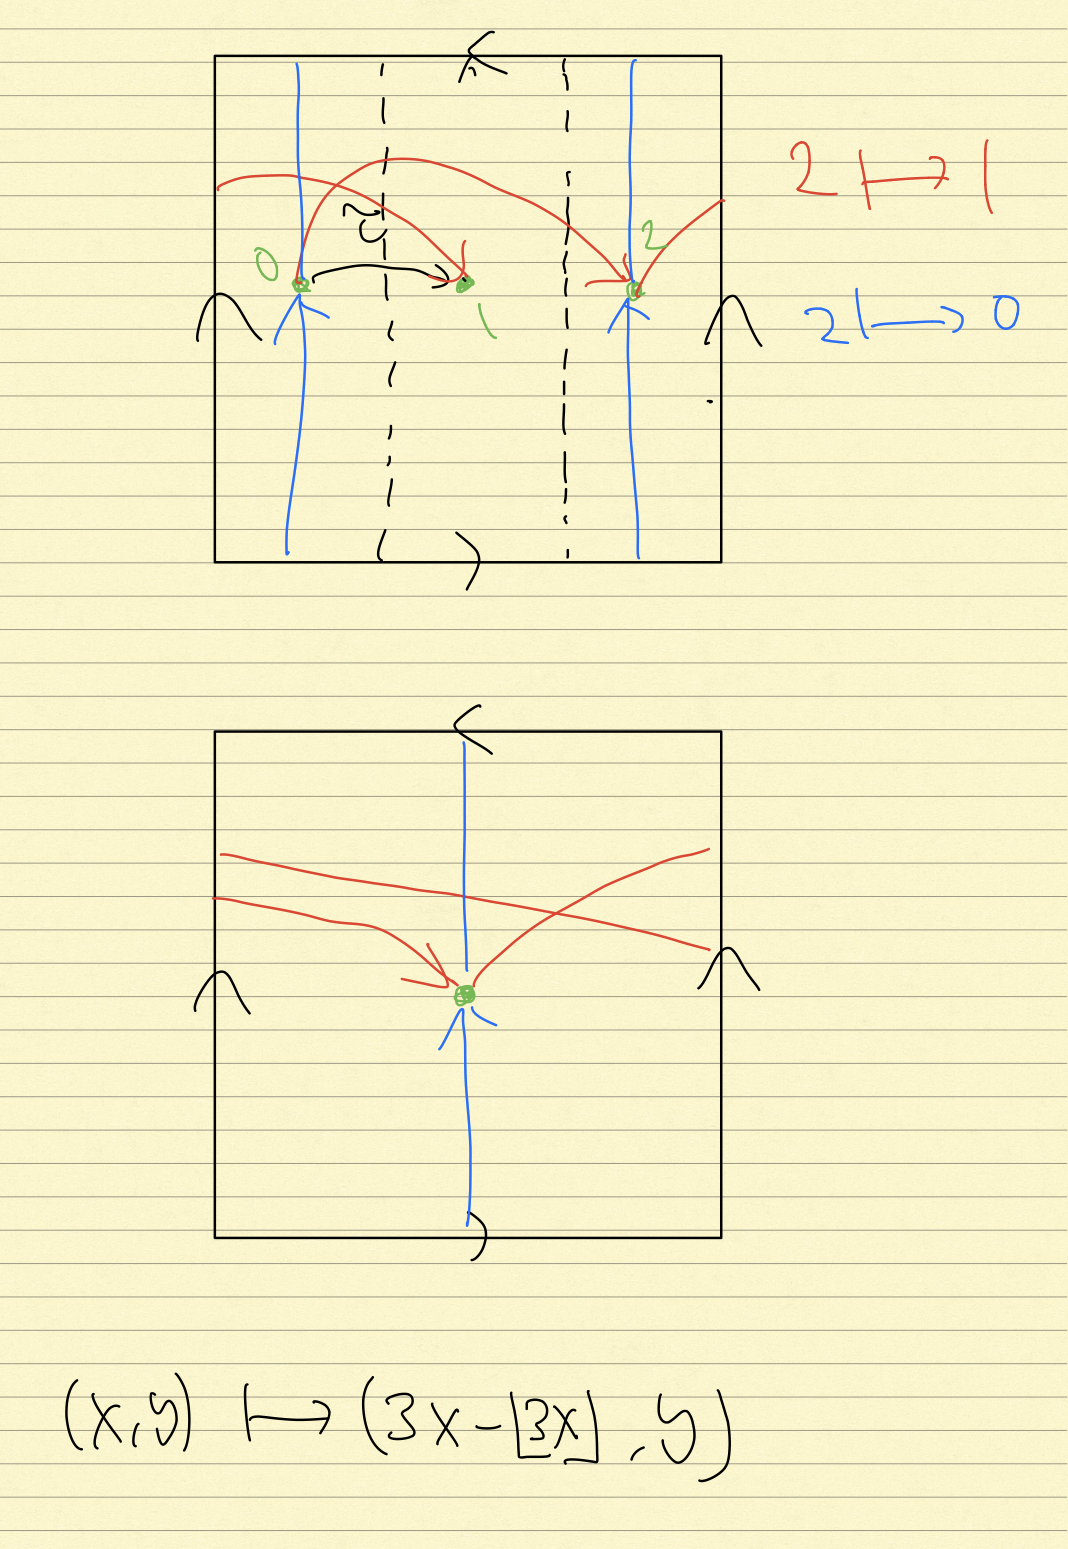
\includegraphics[width=.5\linewidth]{non_normal_covering_klein.jpeg}
    \caption{Problem 20 (Klein)}
    \label{fig:non_normal_covering_klein}
  \end{figure}

  \begin{figure}
    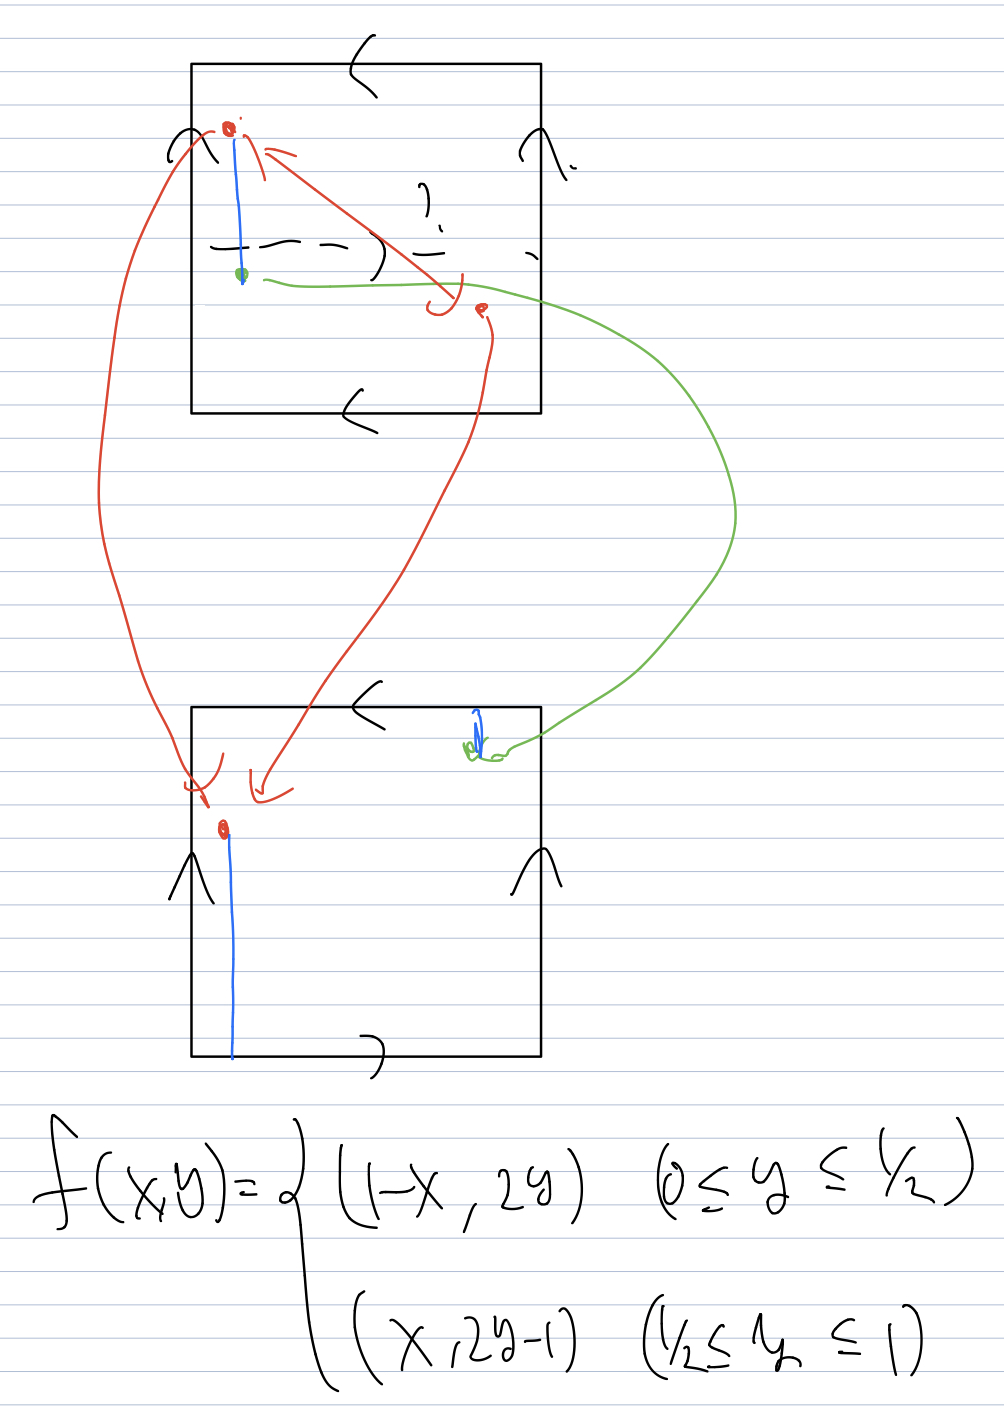
\includegraphics[width=.5\linewidth]{non_normal_covering_torus.jpeg}
    \caption{Problem 20 (Torus)}
    \label{fig:non_normal_covering_torus}
  \end{figure}
  
\end{proof}

\end{document}


